%%%%%%%%%%%%%%%%%%%%%%%%%%%%%%%%%%%%
% Slide options
%%%%%%%%%%%%%%%%%%%%%%%%%%%%%%%%%%%%

% Option 1: Slides with solutions

\documentclass[slidestop,compress,mathserif]{beamer}
\newcommand{\soln}[1]{\textit{#1}}
\newcommand{\solnGr}[1]{#1}

% Option 2: Handouts without solutions

%\documentclass[11pt,containsverbatim,handout]{beamer}
%\usepackage{pgfpages}
%\pgfpagesuselayout{4 on 1}[letterpaper,landscape,border shrink=5mm]
%\newcommand{\soln}[1]{ }
%\newcommand{\solnGr}{ }


%%%%%%%%%%%%%%%%%%%%%%%%%%%%%%%%%%%%
% Style
%%%%%%%%%%%%%%%%%%%%%%%%%%%%%%%%%%%%

\def\chp3@path{../../Chp 3}
\input{../../lec_style.tex}


%%%%%%%%%%%%%%%%%%%%%%%%%%%%%%%%%%%%
% Preamble
%%%%%%%%%%%%%%%%%%%%%%%%%%%%%%%%%%%%

\title[Lecture 9]{MA213: Lecture 9}
\subtitle{Module 2: Probability, Random Variables, and Distributions}
\author{OpenIntro Statistics, 4th Edition}
\institute{$\:$ \\ {\footnotesize Based on slides developed by Mine \c{C}etinkaya-Rundel of OpenIntro. \\
The slides may be copied, edited, and/or shared via the \webLink{http://creativecommons.org/licenses/by-sa/3.0/us/}{CC BY-SA license.} \\
Some images may be included under fair use guidelines (educational purposes).}}
\date{}

%%%%%%%%%%%%%%%%%%%%%%%%%%%%%%%%%%%%
% Begin document
%%%%%%%%%%%%%%%%%%%%%%%%%%%%%%%%%%%%

\begin{document}


%%%%%%%%%%%%%%%%%%%%%%%%%%%%%%%%%%%%
% Title page
%%%%%%%%%%%%%%%%%%%%%%%%%%%%%%%%%%%%

{
\addtocounter{framenumber}{-1} 
{\removepagenumbers 
\usebackgroundtemplate{\includegraphics[width=\paperwidth]{../../OpenIntro_Grid_4_3-01.jpg}}
\begin{frame}

\hfill \includegraphics[width=20mm]{../../oiLogo_highres}

\titlepage

\end{frame}
}
}


%%%%%%%%%%%%%%%%%%%%%%%%%%%%%%%%%%%%
% Recap/Agenda 
%%%%%%%%%%%%%%%%%%%%%%%%%%%%%%%%%%%%
% TODO better formatting
\begin{frame}
    \frametitle{Module 2: Probability, Random Variables, and Distributions}
    \begin{itemize}
        \item \hl{Previously: } Random Variables (Chapter 3.4)
        \item \hl{This time: } Continuous Distributions (Chapter 3.5)
        \item \hl{Reading: } Chapter 4.1 for next time
        \item \hl{Deadlines/Announcements: } Quiz 1 in discussions this week, HW 2.1 due today
    \end{itemize}
    
\end{frame}
    

%%%%%%%%%%%%%%%%%%%%%%%%%%%%%%%%%%%%
% Sections
%%%%%%%%%%%%%%%%%%%%%%%%%%%%%%%%%%%%

\subsection{Recap}

%%%%%%%%%%%%%%%%%%%%%%%%%%%%%%%%%%%%

\begin{frame}
\frametitle{Practice}

\pq{A casino game costs \$5 to play. If the first card you draw is red, then you get to draw a second card (without replacement). If the second card is the ace of clubs, you win \$500. If not, you don't win anything, i.e. lose your \$5. What is your expected profits/losses from playing this game? {\small Remember: profit/loss = winnings - cost.}}

\begin{multicols}{2}
\begin{enumerate}[(a)]
\item A profit of 5\textcent
\solnMult{A loss of 10\textcent}
\item A loss of 25\textcent
\item A loss of 30\textcent
\end{enumerate}
\end{multicols}

\soln{
\only<2>{
{\small
\renewcommand\arraystretch{1.25}
\begin{tabular}{l c c c r}
Event				& Win	& Profit: $X$	& $P(X)$	& $ X \times P(X)$	\\
\hline
\orange{Red}, {A}{$\clubsuit$}		& 500		& 500 - 5 = 495	& $\frac{26}{52} \times \frac{1}{51} = 	0.0098$ & 	 $495 \times 0.0098 = 4.851$ \\
Other	& 0 			& 0 - 5 = -5	& $1 - 0.0098 = 0.9902$ & $-5 \times 0.9902 = -4.951$ \\  
\hline
					&			&			& 			& $E(X) = -0.1$
\end{tabular}
}
}
}

\end{frame}

%%%%%%%%%%%%%%%%%%%%%%%%%%%%%%%%%%%%

\begin{frame}
\frametitle{Fair game}

A \hl{fair} game is defined as a game that costs as much as its expected payout, i.e. expected profit is 0.

\pause

$\:$

\dq{Do you think casino games in Vegas cost more or less than their expected payouts?}

\soln{
\pause
\begin{columns}[c]
\column{0.6\textwidth}
If those games cost less than their expected payouts, it would mean that the casinos would be losing money on average, and hence they wouldn't be able to pay for all this:
\column{0.4\textwidth}
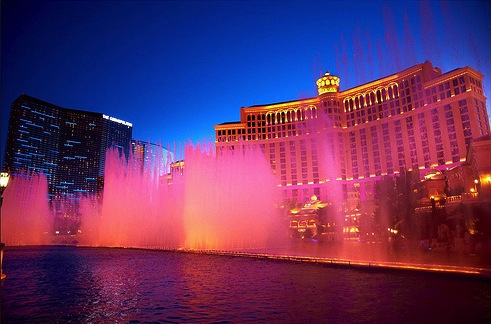
\includegraphics[width=\textwidth]{\chp3@path/3-4_random_variables/figures/bellagio.jpg}
\end{columns}
\ct{Image by Moyan\_Brenn on Flickr \webURL{http://www.flickr.com/photos/aigle\_dore/5951714693}.}
}


\end{frame}

%%%%%%%%%%%%%%%%%%%%%%%%%%%%%%%%%%%%%

\begin{frame}
\frametitle{Simplifying random variables}

Random variables do not work like normal algebraic variables:
\[ X + X \ne 2X \]

\pause

{\small
\twocol{0.45}{0.45}
{
\begin{align*}
E(X + X) &= E(X) + E(X) \\
&= 2 E(X) \\
&~  \\
E(2X) &= 2 E(X) \\
&~ 
\end{align*}
}
{
\begin{align*}
Var(X + X) &= Var(X) + Var(X)~{\scriptsize \text{(assuming independence)}} \\
&= 2~Var(X) \\
&~  \\
Var(2X) &= 2^2~Var(X) \\
&= 4~Var(X)
\end{align*}
}
}


\pause

\vspace{3mm}

\mathhl{E(X + X)  = E(2X)}, but \mathhl{Var(X + X) \ne Var(2X)}.

\end{frame}

%%%%%%%%%%%%%%%%%%%%%%%%%%%%%%%%%%%%%

\begin{frame}
\frametitle{Adding or multiplying?}

\dq{A company has 5 Lincoln Town Cars in its fleet. Historical data show that annual maintenance cost for each car is on average \$2,154 with a standard deviation of \$132. What is the mean and the standard deviation of the total annual maintenance cost for this fleet?}

\pause

Note that we have 5 cars each with the given annual maintenance cost $(X_1 + X_2 + X_3 + X_4 + X_5)$, not one car that had 5 times the given annual maintenance cost $(5X)$.

\pause

{\small
\begin{eqnarray*} 
E(X_1 + X_2 + X_3 + X_4 + X_5) &=& E(X_1) + E(X_2) + E(X_3) + E(X_4) + E(X_5) \\
\pause
&=& 5 \times E(X) = 5 \times 2,154 = \$ 10,770 \\
\pause
Var(X_1 + X_2 + X_3 + X_4 + X_5) &=& Var(X_1) + Var(X_2) + Var(X_3) + Var(X_4) + Var(X_5) \\
\pause
&=& 5 \times V(X) = 5 \times 132^2 = \$ 87,120 \\
\pause
SD(X_1 + X_2 + X_3 + X_4 + X_5) &=& \sqrt{87,120} =  295.16
\end{eqnarray*}
}

\end{frame}

%%%%%%%%%%%%%%%%%%%%%%%%%%%%%%%%%%%%

\section{Continuous distributions}

%%%%%%%%%%%%%%%%%%%%%%%%%%%%%%%%%%%%

\begin{frame}
\frametitle{Continuous distributions}

\begin{itemize}

\item Below is a histogram of the distribution of heights of US adults. 

\item The proportion of data that falls in the shaded bins gives the probability that a randomly sampled US adult is between 180 cm and 185 cm (about 5'11" to 6'1").

\end{itemize}

\begin{center}
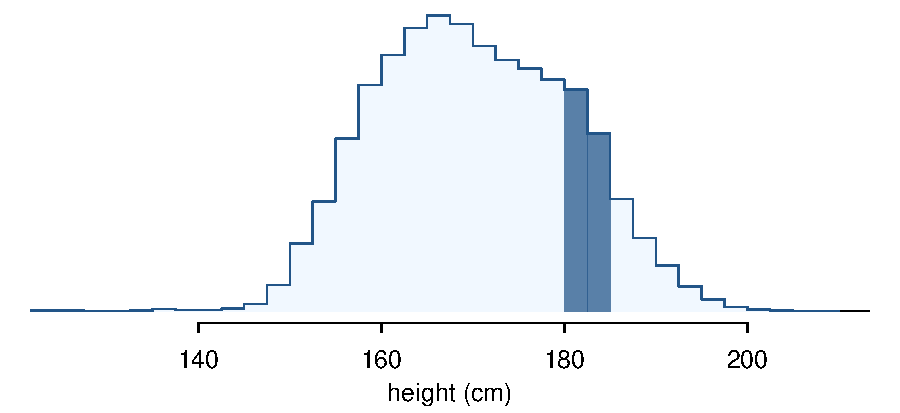
\includegraphics[width=\textwidth]{\chp3@path/3-5_continuous_distributions/figures/usHeightsHist180185/usHeightsHist180185}
\end{center}


\end{frame}

%%%%%%%%%%%%%%%%%%%%%%%%%%%%%%%%%%%%

\subsection{From histograms to continuous distributions}

\begin{frame}
\frametitle{From histograms to continuous distributions}

Since height is a continuous numerical variable, its \hl{probability density function} is a smooth curve.

\begin{center}
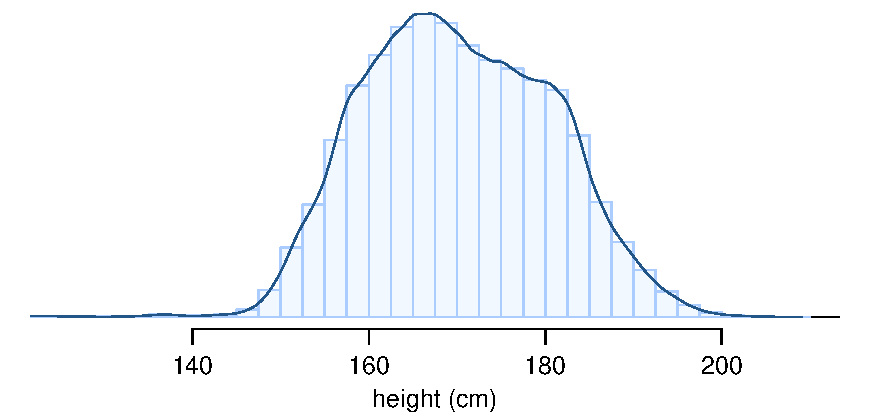
\includegraphics[width=\textwidth]{\chp3@path/3-5_continuous_distributions/figures/fdicHeightContDist/fdicHeightContDist}
\end{center}

\end{frame}

%%%%%%%%%%%%%%%%%%%%%%%%%%%%%%%%%%%%

\subsection{Probabilities from continuous distributions}

\begin{frame}
\frametitle{Probabilities from continuous distributions}

Therefore, the probability that a randomly sampled US adult is between 180 cm and 185 cm can also be estimated as the shaded area under the curve.

\begin{center}
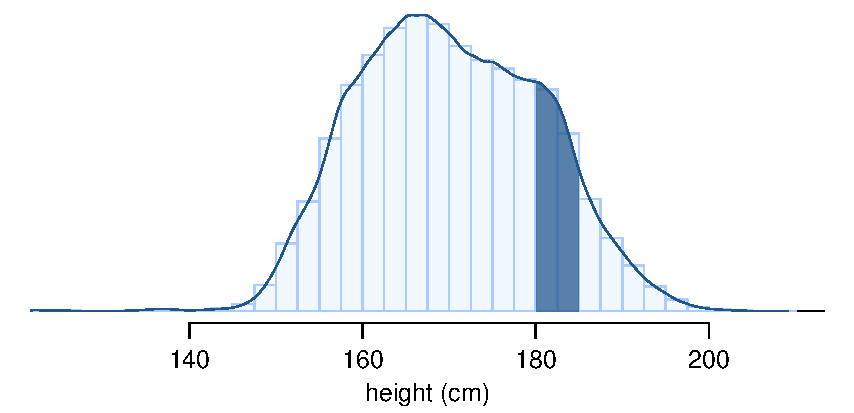
\includegraphics[width=\textwidth]{\chp3@path/3-5_continuous_distributions/figures/fdicHeightContDistFilled/fdicHeightContDistFilled}
\end{center}


\end{frame}

%%%%%%%%%%%%%%%%%%%%%%%%%%%%%%%%%%%%

\begin{frame}
\frametitle{By definition...}

Since continuous probabilities are estimated as ``the area under the curve", the probability of a person being exactly 180 cm (or any exact value) is defined as 0.

\begin{center}
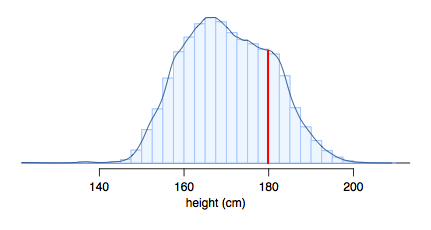
\includegraphics[width=0.8\textwidth]{\chp3@path/3-5_continuous_distributions/figures/fdicHeightContDist180}
\end{center}

\end{frame}

%%%%%%%%%%%%%%%%%%%%%%%%%%%%%%%%%%%%

\section{R Demonstration}

%%%%%%%%%%%%%%%%%%%%%%%%%%%%%%%%%%%%

\section{Edfinity quiz}

%%%%%%%%%%%%%%%%%%%%%%%%%%%%%%%%%%%%

%%%%%%%%%%%%%%%%%%%%%%%%%%%%%%%%%%%%
% End document
%%%%%%%%%%%%%%%%%%%%%%%%%%%%%%%%%%%%

\end{document}